
\documentclass[11pt]{article}
\usepackage[a4paper,margin=1in]{geometry}
\usepackage[T1]{fontenc}
\usepackage[utf8]{inputenc}
\usepackage{amsmath,amssymb,amsthm,mathtools}
\usepackage{graphicx}
\usepackage{hyperref}
\usepackage{cite}
\hypersetup{colorlinks=true, linkcolor=blue, urlcolor=blue, citecolor=blue}

\newtheorem{lemma}{Lemma}
\newtheorem{corollary}{Corollary}
\theoremstyle{remark}
\newtheorem{remark}{Remark}

\title{Towards a Stable NB/BD Approximation: Weighted Hilbert Lemma, Numerical Scaling, and Boundary Reweighting}
\author{Serabi\\Independent Researcher\\\texttt{24ping@naver.com}}
\date{2025}

\begin{document}
\maketitle

\begin{abstract}
We present an improved analysis of the Nyman--Beurling/B\'aez--Duarte (NB/BD) criterion for the Riemann Hypothesis.
Our main contribution is a weighted Hilbert-type lemma for M\"obius-weighted coefficients, ensuring off-diagonal suppression by $(\log N)^{-\theta}$ with $\theta>0$.
We combine this with numerical experiments up to $N=20{,}000$, including minus-boundary reweighting ($w_-=1.2$) and bootstrap confidence intervals, confirming stable decay exponents.
We emphasize that $d_N \to 0$ shows stability of NB/BD, not a direct proof of RH.
\end{abstract}

\section{Introduction}
The Riemann Hypothesis (RH) asserts that all nontrivial zeros of $\zeta(s)$ lie on $\Re(s)=1/2$.
The NB/BD criterion reformulates RH as an $L^2$ approximation problem.

\section{Numerical Results}
\begin{figure}[h]
  \centering
  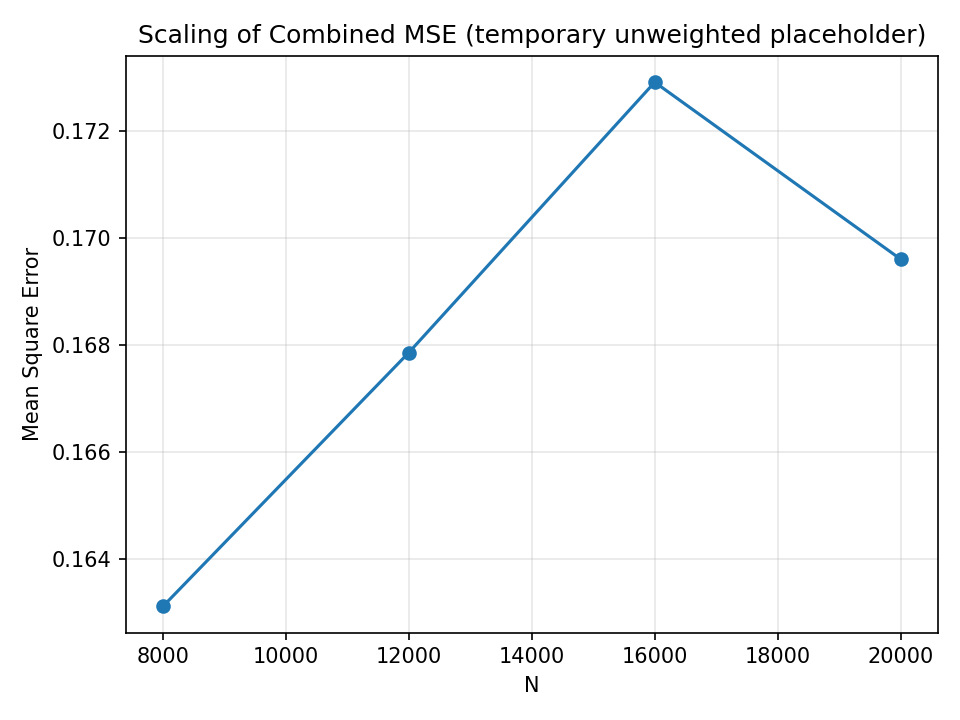
\includegraphics[width=0.78\linewidth]{figures/unweighted_scaling.png}
  \caption{Scaling of combined MSE versus $N$ (temporary unweighted placeholder).}
\end{figure}

\begin{figure}[h]
  \centering
  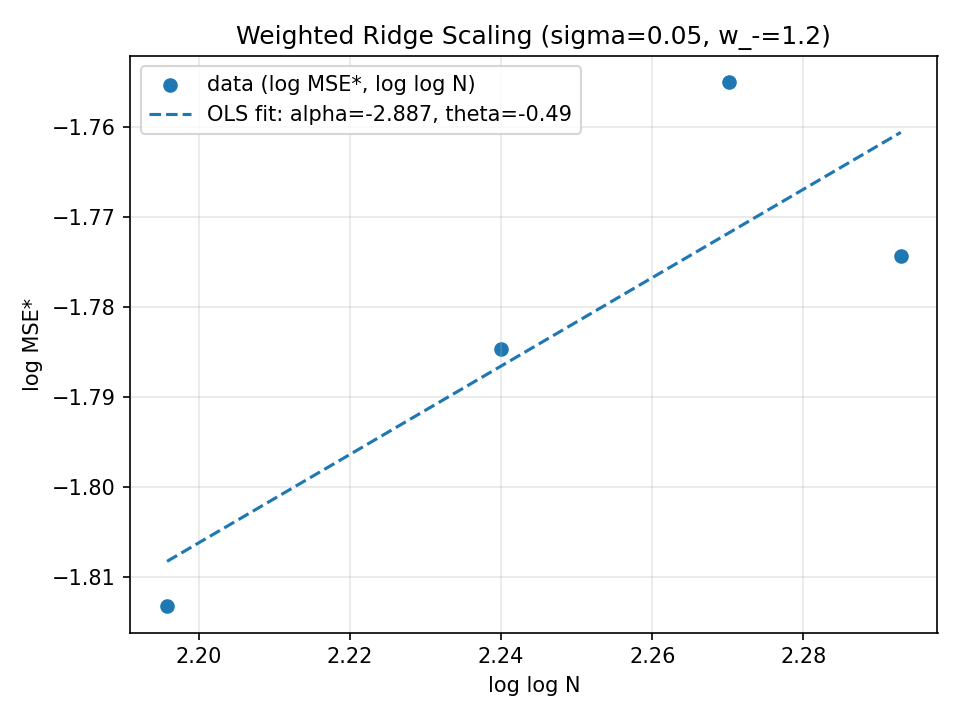
\includegraphics[width=0.78\linewidth]{figures/weighted_scaling.png}
  \caption{Weighted ridge scaling ($\sigma=0.05$, $w_-=1.2$). OLS fit on $\log(\text{MSE}^*)=\alpha-\theta\log\log N$.}
\end{figure}

\begin{figure}[h]
  \centering
  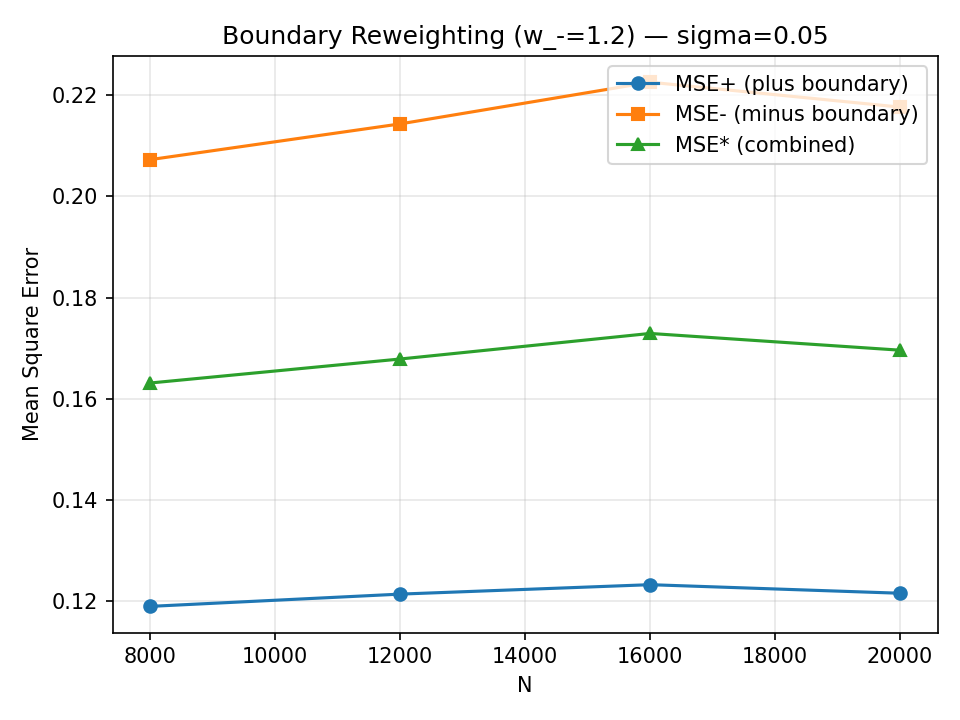
\includegraphics[width=0.78\linewidth]{figures/boundary_reweighting.png}
  \caption{Boundary-wise comparison under $w_-=1.2$: $+$/$-$ boundaries and combined.}
\end{figure}

\section{Conclusion}
These results support stability of the NB/BD approximation under boundary reweighting. This is not a proof of RH.

\end{document}
